\section{Implementation}

In this section we present the implementation of our algorithm and compare it with the conventional unification algorithm used in most \miniKanren implementations
(which is in turn based on Robinson's algorithm with triangular substitutions~\cite{baader2001unification}). Specifically, we consider a simplified version of \OCanren
unification implementation.

In both algorithms the datatype for the state is a mapping from variables to terms:

\begin{minted}{OCaml}
module Term = struct
  type t =
  | Var of int
  | Con of int * t array
end
module M = Map.Make(Int)
\end{minted}

The difference is in the interpretation of this intermediate state. While in conventional unification we understand an intermediate state as a substitution $\sigma$ (encoded
in a triangular manner~\cite{baader2001unification}), in rational unification we understand it as an equation system $\xi$ encoded in a union-find manner~\cite{arden1961algorithm}\footnote{Actually, we don't use path-compression and rank heuristic since they slow down the algorithm in persistent implementations. Thus, it may be called ``a triangular equation system''.}.

The core operation \walk which allows us to ``dereference'' variables in triangular substitution changes its signature from $\walk : \Sigma \times \V \rightarrow T$ to $\walk : \Xi \times \V \rightarrow \E \times T$ and plays the role of the ``find'' operation of union-find:

\begin{center}
    \begin{minipage}{0.46\textwidth}
        \centering
        \begin{minted}[fontsize=\small,baselinestretch=0.9]{OCaml}
let rec walk s x = match M.find x s with
| exception Not_found -> Term.Var x
| Term.Var x -> walk s x
| t -> t
        \end{minted}
    \end{minipage}
    \hfill
    \vrule
    \hfill
    \begin{minipage}{0.46\textwidth}
        \centering
        \begin{minted}[fontsize=\small,baselinestretch=0.9]{OCaml}
let rec walk s x = match M.find x s with
| exception Not_found -> x, Term.Var x
| Term.Var x -> walk s x
| t -> x, t
        \end{minted}
    \end{minipage}
\end{center}

The only difference is an ability to observe the ``final'' variable in a ``dereference'' chain. In implementation, we deal with representing variables instead of equations defined in the previous section.

Let us recall the ``occurs check'' from the conventional algorithm:

\begin{minted}{OCaml}
let rec occurs s x = function
| Term.Var y ->
  begin match walk s y with
  | Term.Var y -> if x == y then raise Occurs
  | t -> occurs x t
  end
| Term.Con (_, ts) -> Array.iter (occurs s x) ts

let extend s x t = occurs s x t ; M.add x t s
\end{minted}

While in the conventional algorithm these functions help us to prevent the construction of illegal (recursive) substitution, rational unification don't rely on them.

Instead, we define the operations $\commonpart : T \times T \rightarrow T^?$ and $\union : \Xi \times \V \times \V \rightarrow \Xi \times (T \times T)^?$:

\begin{minted}{OCaml}
module Term = struct
  let rec common_part x y = match x, y with
  | Var x, _ -> Var x
  | _, Var y -> Var y
  | Con (f, ts1), Con (g, ts2)
  when f == g && Array.length ts1 == Array.length ts2 ->
    Con (f, Array.map2 common_part ts1 ts2)
  | _ -> raise No_common_part
end

let union s x y =
  let x, xt = walk s x in
  let y, yt = walk s y in
  if x == y then s, None
  else begin match xt, yt with
  | Var _, Var _ -> M.add x yt s, None
  | Var _, _ -> M.add x (Term.Var y) s, None
  | _, Var _ -> M.add y (Term.Var x) s, None
  | _, _ -> M.add x (Term.Var y) s, Some (xt, yt)
  end
\end{minted}

Finally, we implement the algorithm itself:

\begin{center}
    \begin{minipage}{0.46\textwidth}
        \centering
        \begin{minted}[fontsize=\small,baselinestretch=0.9]{OCaml}
let rec unify_vt s x yt =
  match walk s x with
  | Term.Var x -> extend s x yt
  | xt -> unify xt yt

and unify s xt yt =
  if xt == yt then s
  else match xt, yt with
  | Term.Var x, Term.Var y ->
    begin match walk s x, walk s y with
    | Term.Var x, Term.Var y ->
      M.add x (Term.Var y) s
    | Term.Var x, yt -> extend s x yt
    | xt, Term.Var y -> extend s y xt
    | xt, yt -> unify s xt yt
    end
  | Term.Var x, _ -> unify_vt s x yt
  | _, Term.Var y -> unify_vt s y xt
  | Term.Con (f, ts1), Term.Con (g, ts2)
  when f == g && Array.length ts1
              == Array.length ts2 ->
    let n = Array.length ts1 in
    let rec hlp i s =
      if i == n then s
      else hlp (i + 1)
        @@ unify s ts1.(i) ts2.(i)
    in
    hlp 0 s
  | _ -> raise Term.No_common_part
        \end{minted}
    \end{minipage}
    \hfill
    \vrule
    \hfill
    \begin{minipage}{0.46\textwidth}
        \centering
        \begin{minted}[fontsize=\small,baselinestretch=0.9]{OCaml}
let rec unify_vt s x yt =
  let x, xt = walk s x in
  begin match xt with
  | Term.Var _ -> M.add x yt s
  | _ ->
    let t = Term.common_part xt yt in
    unify (M.add x t s) xt yt
  end

and unify s xt yt =
  if xt == yt then s
  else match xt, yt with
  | Term.Var x, Term.Var y ->
    begin match union s x y with
    | s, Some (xt, yt) -> unify s xt yt
    | s, None -> s
    end
  | Term.Var x, _ -> unify_vt s x yt
  | _, Term.Var y -> unify_vt s y xt
  | Term.Con (f, ts1), Term.Con (g, ts2)
  when f == g && Array.length ts1
              == Array.length ts2 ->
    let n = Array.length ts1 in
    let rec hlp i s =
      if i == n then s
      else hlp (i + 1)
        @@ unify s ts1.(i) ts2.(i)
    in
    hlp 0 s
  | _ -> raise Term.No_common_part
        \end{minted}
    \end{minipage}
\end{center}

While handling the two-constructors case is the same, the changes affect other cases:

\begin{itemize}
    \item The logic of unification of two variables completely migrates in \union.
    \item The logic of unification of a variable and a constructor-term is incorporated in the \commonpart call. 
\end{itemize}

With these changes we may see that the unification of two variables now always assigns a variable to a variable.
For example, if $x$ is bound to $f\,(y)$ the result of conventional unification of $x$ and $z$ includes the binding $z \mapsto f\,(y)$ while the result of our unification includes $z \mapsto x$.
Also, \union performs ``eager'' binding of variables, i.e., if $x$ is bound to $f\,(v)$ and $y$ is bound to $f\,(u)$ the result of conventional unification of $x$ and $y$ includes the binding $v \mapsto u$ and not $x \mapsto y$ while the result of our unification includes both.

The usage of \commonpart forces the unification algorithm to decompose ``complex'' terms in an equation system.
For example, if $x$ is bound to $f\,(g\,(y))$, the result of conventional unification of $x$ and $f\,(z)$ includes $x \mapsto f\,(g\,(y)), z \mapsto g\,(y)$ while the result of our unification includes $x \mapsto f\,(z), z \mapsto g\,(y)$ instead.

While these changes are required to prevent infinite looping and provide the correctness of the algorithm, they abuse variables reassigning in intermediate states.
This makes it more complicated to apply scope-based optimization~\cite{byrd2009relational} widely used in \miniKanren implementations. More precisely, we need to check a substitution in a state before an attribute one -- since it seems too wasteful, in practice, substitutions in states become noticeably small in presence of the optimization so the performance degradation is acceptable (based on some experiments and not verified strictly).

The crucial optimization for the presented algorithm is the well-known variable-age heuristic~\cite{mannila1986complexity,domoratskiy2025empirical} which reduces \walk paths, and it applies directly on \union.

\subsection{Optimized Common Part}

A notable optimization is the implementation of \commonpart which preserves ``physical equality''\footnote{``Physical equality'' is the equality of the references to the objects in memory.} as long as possible. The optimization is motivated by both a reduction of memory consumption and an efficiency improving of the unification itself (since we may do a fail-fast ``physical equality'' check).

The core idea is to consider a simple lattice of four elements (we name it ``side''): $\top$~(\texttt{Both}), $\Leftarrow$~(\texttt{Left}), $\Rightarrow$~(\texttt{Right}) and $\bot$~(\texttt{Aside}):
\begin{center}
    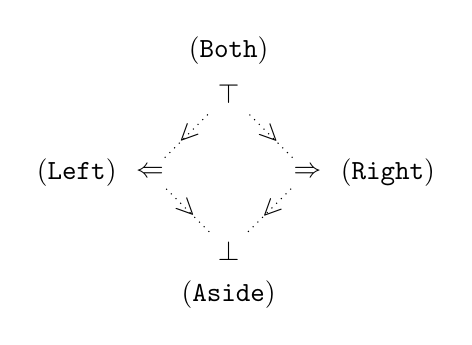
\begin{tikzpicture}
        \node (both) at (0, 1) {$\top$};
        \node (left) at (-1, 0) {$\Leftarrow$};
        \node (right) at (1, 0) {$\Rightarrow$};
        \node (aside) at (0, -1) {$\bot$};
        \draw[dotted] (left) -- (both) node[midway,sloped] {$<$};
        \draw[dotted] (right) -- (both) node[midway,sloped] {$>$};
        \draw[dotted] (aside) -- (left) node[midway,sloped] {$>$};
        \draw[dotted] (aside) -- (right) node[midway,sloped] {$<$};
        \node[anchor=south] at (both.north) {(\texttt{Both})};
        \node[anchor=east] at (left.west) {(\texttt{Left})};
        \node[anchor=west] at (right.east) {(\texttt{Right})};
        \node[anchor=north] at (aside.south) {(\texttt{Aside})};
    \end{tikzpicture}
\end{center}

This lattice designates which of the arguments are ``physically equal'' to their \commonpart. With it, the optimization is captured by the function $\commonpart' : T \times T \rightarrow (T \times \textsf{Side})^?$. Since non-recursive cases are trivial, while performing recursive calls we are accumulating a supremum of sides:
\begin{itemize}
    \item if it is $\bot$, we are required to return the accumulated term (as in a straightforward implementation) -- there is no way to preserve a ``physical equality'' to any of the arguments;
    \item otherwise, we are discarding the accumulated term and return one of the arguments instead.
\end{itemize}

The implementation is mostly intuitive but verbose, so we omit it and refer to the repository with evaluation of the algorithm. Also, we haven't measured the concrete performance impact of this algorithm w.r.t. the simple one.
